\chapter{Week 5: 20\textsuperscript{th}  - 26\textsuperscript{th} Oct}


 \tocless\section{Objectives}
\begin{itemize}
	\item Find the moments of inertia of the about all three axes.
\end{itemize}

 \tocless\section{Inertia about each axis}
To find the moment of inertia of the quad-rotor the rig was held by cable  at it's end point and allowed to swing about a single axis. To document the amplitude of the quad-rotor at each oscillation a laser pointer was attached to the end of the quad-rotor \footnote{This was done so one could acquire the damping of the system about each axis after the test was completed}and to record the period of each oscillation a stop watch \footnote{This was done so one could a quire the moment of inertia about each axis}. The oscillation was carried out about a low friction surface to ensure an accurate value for the moment of inertia of each axis. The results were entered into Matlab and the following results were acquired for the moment of inertia of the system.


\begin{align}
I =  
\begin{bmatrix}
\gls{interiaofroll}  & 0 & 0 \\ 0& \gls{interiaofpitch} & 0 \\0& 0& \gls{interiaofyaw}
\end{bmatrix}
=
\begin{bmatrix}
0.1274 & 0 & 0 \\ 0& 0.1221& 0 \\0& 0& 0.2370
\end{bmatrix}
\label{eq: moment of interia of the system}
\end{align} 



Note as the system is symmetric about the pitch and roll axis one can assume that $\gls{interiaofroll}   =\approx \gls{interiaofpitch}$.

 \tocless\section{Damping}

 The results for the maximum amplitude were processed using Matlab and the results were plotted yielding figure \ref{fig: plot of angle vs time}.
\begin{figure}[t]
	\centering
	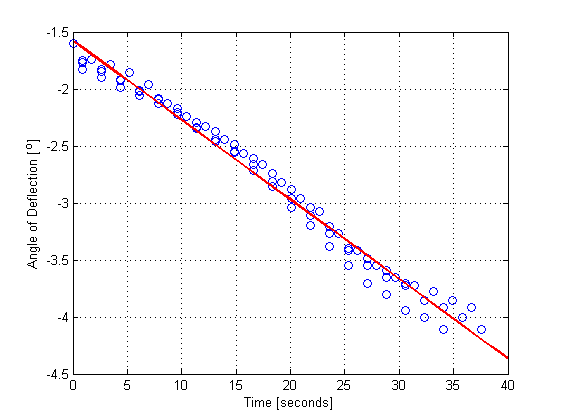
\includegraphics[scale = 1]{\DocRoot/images/moment_inertia}
	\caption{Plot of deflection from normal  vs Time}
	\label{fig: plot of angle vs time}
\end{figure}

From figure \ref{fig: plot of angle vs time} one can acquire the moment of inertia from the slope of the line and thus define the inertia of the system as follows. 

\begin{align}
\beta =  
\begin{bmatrix}
\gls{dampingroll}  & 0 & 0 \\ 0& \gls{dampingpitch} & 0 \\0& 0& \gls{dampingyaw}
\end{bmatrix}
=
\begin{bmatrix}
 0.0194 & 0 & 0 \\ 0&  0.0194 & 0 \\0& 0&  \approx 0
\end{bmatrix}
\label{eq: damping of the system}
\end{align} 
